\documentclass[11pt]{article}
\usepackage[paperwidth=8.5in, paperheight=11in]{geometry}

\usepackage{../tjimo}

%\begin{comment}
\def\answer{\comment}
\def\solution{\comment}
\def\solutionone{\comment}
\def\solutiontwo{\comment}
%\end{comment}

\newcommand{\sevenpoints}{Time limit: 30 minutes.}
\newcommand{\righthead}{\fdbox{Round}{Practice Team}}

\begin{document}

\begin{problem}
% (1) (2016skim) 
There are 2015 potatoes in a basket. If you can only take out 11 at a time, what is the minimum number of potatoes you can leave in the basket?
\end{problem}

\begin{answer}
\boxed{2}.
\end{answer}

\begin{solution}
This is simply finding the remainder when dividing 2015 by 11, which is \boxed{2}.
\end{solution}

\begin{problem}
% (1.5) (2016skim) 
A $8 \times 8 \times 8$ cube is cut up into unit cubes, and one is randomly removed. What is the probability that the cube still looks the same from the outside? (Ignore the effects of gravity, i.e. cubes will stay floating.)
\end{problem}

\begin{answer}
\boxed{\frac{27}{64}}.
\end{answer}

\begin{solution}
One of the inner cubes must be removed for the outside to still look the same. Thus, the probability is $\frac{6^3}{8^3} = \boxed{\frac{27}{64}}$.
\end{solution}

\begin{problem}
% (2) (2016azhang) 
Candide has 120 pieces of candy. In how many ways can Candide split all of his candies into equally sized pile(s)? (Two examples are 1 pile of 120 pieces, and 20 piles of 6 pieces.)
\end{problem}

\begin{answer}
\boxed{16}.
\end{answer}

\begin{solution}
Note that the number of piles (or the number of pieces in a pile) can only be a factor of 120. Since each number of piles leads to a unique pile distribution, our answer is just the number of factors of $120 = 2^{3}\cdot3\cdot5$, which is $(3+1)(1+1)(1+1) = \boxed{16}$.
\end{solution}

\begin{problem}
% (1.5) (2016skim) 
What is the area of the figure below, if it is made up of two overlapping squares of side length 10?
\begin{center}
\begin{asy}
size(5cm);
draw((1,0)--(11,0)--(11,10)--(10,10)--(10,11)--(0,11)--(0,1)--(1,1)--cycle, linewidth(1.5));
label("1", (1,1), SW);
label("10", (6, 0), S);
label("10", (0, 6), W);
\end{asy}
%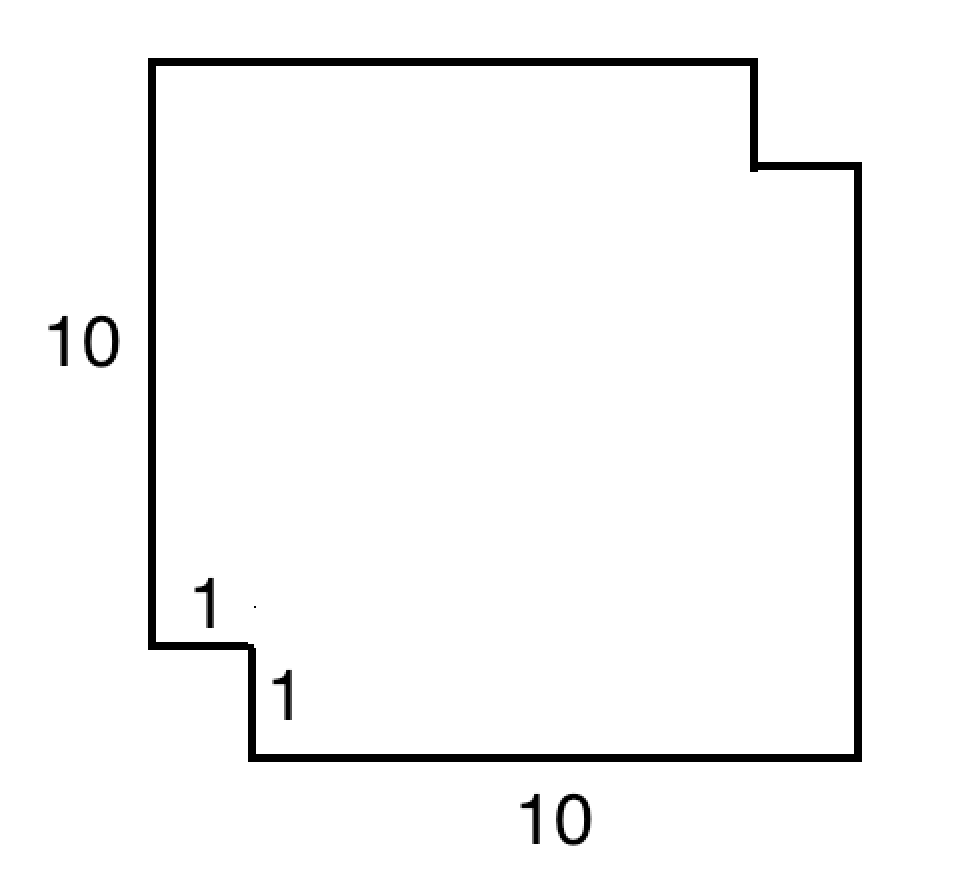
\includegraphics[width=6cm]{squares.png}
\end{center}
\end{problem}

\begin{answer}
\boxed{119}.
\end{answer}

\begin{solution}
We can view this as a $11\times11$ square with 2 unit squares cut off at the corners. The total area is $(11)(11)-2(1) = \boxed{119}$.
\end{solution}

\begin{problem}
% (3) (2016azhang) 
Lilian and Katherine are both expert moppers, and after a gust of wind swept through a mathematics room at CMU, they volunteered to sweep up the 100 math problems now on the floor. Of the 100 math problems, 50 of them involved algebra, 30 involved geometry, and 12 involved both algebra and geometry. Out of curiosity, they randomly picked up a problem on the floor and read it. Given that the problem did not involve both algebra and geometry, what is the probability that the problem involved algebra?
\end{problem}

\begin{answer}
\boxed{\frac{19}{44}}.
\end{answer}

\begin{solution}
We can split up the problem types into 4 categories: Involving both algebra and geometry, involving algebra but not geometry, involving geometry but not algebra, and involving neither algebra nor geometry. Since 12 problems involved both algebra and geometry, that means that $50-12 = 38$ problems involved algebra but not geometry, and $30-12 = 18$ problems involved geometry but not algebra. This leaves $100 - 38 - 18 - 12 = 32$ problems involving neither algebra nor geometry. Since we are given that the problem did not involve both algebra and geometry, we exclude those 12 problems from our probability space, and our desired probability is thus $\frac{38}{88}$ = \boxed{\frac{19}{44}}.
\end{solution}

\begin{problem}
% (2.5-3) (2016azhang) 
TJHSST is currently selling biology, chemistry, and physics textbooks. Bary-Centric the biologist buys 3 biology, 1 chemistry, and 1 physics textbook for \$100. Carrie the chemist buys 1 biology, 3 chemistry, and 1 physics textbook for \$200. Finally, Parry the physicist buys 1 biology, 1 chemistry, and 3 physics textbooks for \$300. How many cents does 1 biology, 1 chemistry, and 1 physics textbook cost?
\end{problem}

\begin{answer}
\boxed{15000}.
\end{answer}

\begin{solution}
Letting b = the cost of a biology textbook in dollars, c = the cost of a chemistry textbook in dollars, and p = the cost of a physics textbook in dollars, we have the three equations $3b + c + p = 100$, $b + 3c + p = 200$, and $b + c + 3p = 300$. Adding up the three equations gets us $4b + 4c + 4p = 600$, or $b + c + p = 150$. However, we want the cost of $b + c + p$ in cents, so we multiply \$150 by 100 to get \boxed{15000} cents.
\end{solution}

\begin{problem}
%(2.5) (2016skim) 
A, B, C, D, E, and F want to sit at a round table with 6 equally spaced out seats. However, A and B cannot sit directly across each other. If the rotation of the table doesn't matter (ABCDEF is identical to BCDEFA), how many ways are there for the 6 people to sit?
\end{problem}

\begin{answer}
\boxed{96}.
\end{answer}

\begin{solution}
Let's consider the people in order. A can sit anywhere, so there are 6 ways. B can only sit in the seats not directly across A, so there are 4 ways. The other people can sit anywhere, so there are $4*3*2*1 = 24$ ways. However, since rotation doesn't matter, we overcounted by a factor of $6$, meaning that we need to divide by $6$ at the end, giving us $6*4*24/6 = 96$ total ways.
\end{solution}

\begin{problem}
% (3-3.5) (2016azhang) 
The figure below shows an isosceles triangle ABC and its inscribed circle O. Given that OD = 3 and AE = 4, where D is the midpoint of BC and E is the point of tangency of the circle with side AC, find OC. Express your answer in simplest radical form. (Note: Figure not drawn to scale.)
%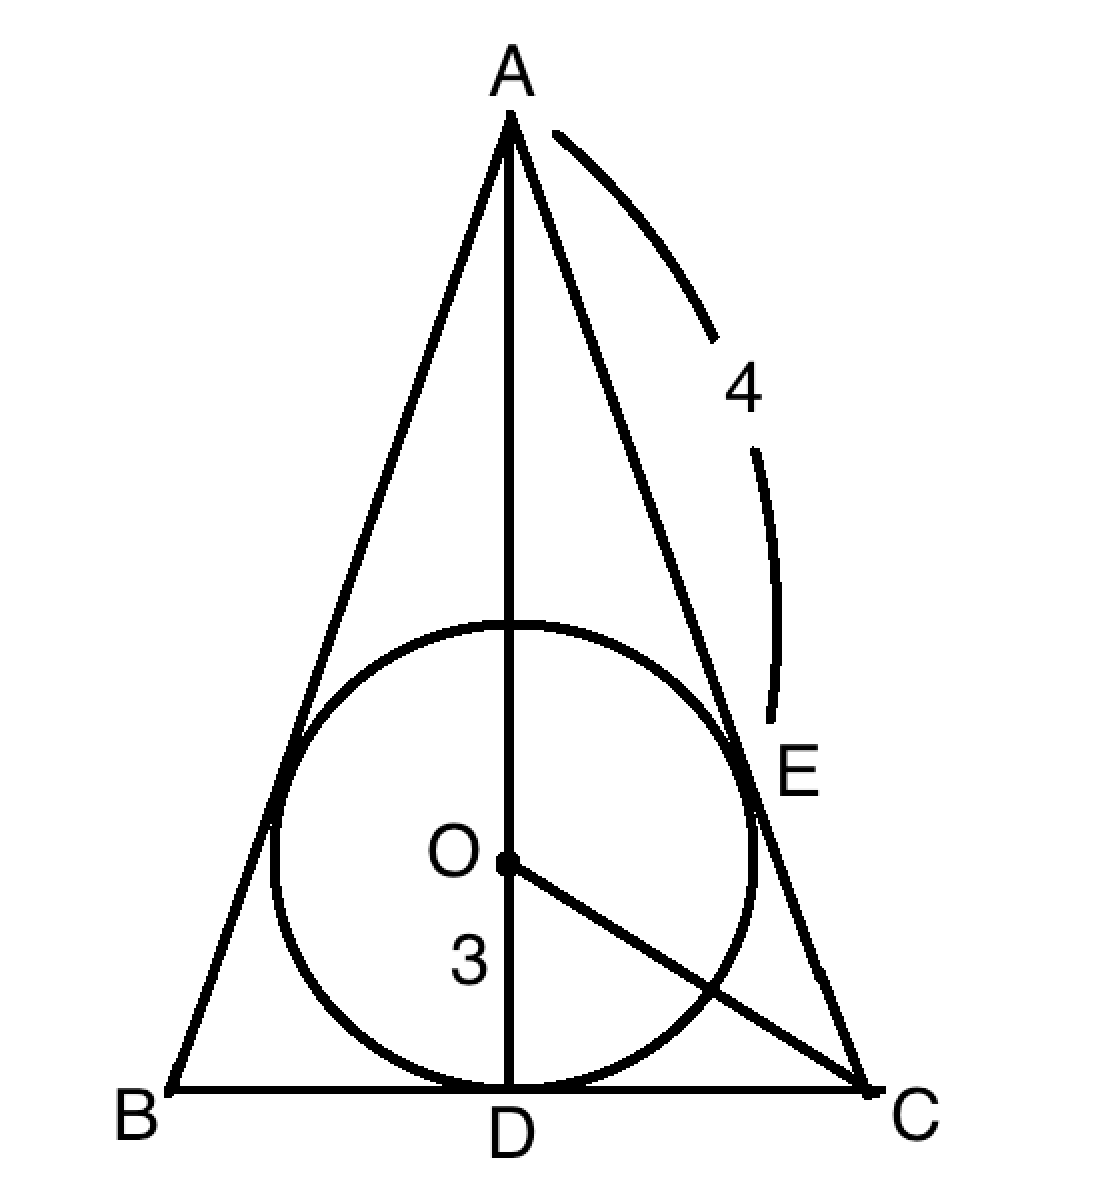
\includegraphics[width=6cm]{triangle.png}
\begin{center}
\begin{asy}
import graph;
size(6cm);
pair A=(0, 8), B=(-6, 0), C=(6,0), D=(0, 0);
draw(A--B--C--cycle, linewidth(1.5));
draw(A--D, linewidth(1.5));
draw(Circle((0, 3), 3), linewidth(1.5));
draw((0,3)--C, linewidth(1.5));

dot((0, 3));

label("$A$", A, NW);
label("$B$", B, W);
label("$C$", C, E);
label("$D$", D, S);
label("$O$", (0, 3), W);
label("$E$", (2.4, 4.8), E);

label("3", (0, 1.5), W);
label("4", (1.2, 6.4), NE);
\end{asy}
\end{center}
\end{problem}

\begin{answer}
\boxed{3\sqrt{5}}.
\end{answer}

\begin{solution}
Note that line segments OE and AC are perpendicular, and line segments BC and AD are perpendicular, as both D and E are points of tangency. Thus, by the Pythagorean Theorem on triangle AOE, we find that AO = 5. Next, note that triangles AOE and ACD are similar, so we have that $\frac{OE}{EA} = \frac{3}{4} = \frac{CD}{DA} = \frac{CD}{3+5} = \frac{CD}{8}$. Thus, $\frac{3}{4} = \frac{CD}{8}$, so CD = 6. Finally, applying the Pythagorean Theorem on triangle ODC gives OC = \boxed{3\sqrt{5}}.
\end{solution}

\begin{problem}
% (3-3.5) (2016azhang) 
Archer is currently doing target practice. Archer is also extremely accurate, as he has a $\frac{9}{10}$ chance of hitting the bulls-eye of a target. If Archer has set up 3 targets for himself, what is the chance that he will only hit 1 bulls-eye of a target?
\end{problem}

\begin{answer}
\boxed{\frac{27}{1000}}.
\end{answer}

\begin{solution}
Let Y represent the event that Archer hits a bulls-eye of one target, and N represent the event that Archer does not hit the bulls-eye of that target. Then we have three possible courses of events where Archer only hits one bulls-eye: YNN, NYN, and NNY. The probability of each event is $\frac{9}{10}\cdot(\frac{1}{10})^2 = \frac{9}{1000}$, and adding up the probabilities gives $3\cdot\frac{9}{1000} = \boxed{\frac{27}{1000}}$.
\end{solution}

\begin{problem} Winston and Allen are playing a game with Allen's collection of 2015 tennis racquets that are numbered from 1 to 2015. Allen will choose a tennis racquet at random and will tell Winston the number of factors of 5 it has. Winston wins if he correctly guesses the number on the tennis racquet given what Allen tells him. If Winston guesses one of the racquets which agrees with Allen's statement, what is the probability that Winston will guess the right racquet number? 
\end{problem}
\begin{answer}
$\boxed{\frac{1}{403}}$
\end{answer}
\begin{solution} We make one important observation. Given any number of factors of 5 Allen gives, say there are $x$ numbers which satisfy this number of factors. If Winston guesses one of these $x$ racquets, he has a $\frac{1}{x}$ probability of guessing the right racquet. We note that there is a $\frac{x}{2015}$ chance of Allen picking a racquet which has that certain number of factors. Therefore, for any number of factors of 5 that Allen picks, there should be a $\frac{1}{x} \times \frac{x}{2015} = \frac{1}{2015}$ chance of picking the right racquet. 

The minimum number of factors of 5 possible is 0. The maximum, in this case, is 4 factors of 5, because $625$, $1250$, and $1875$ have 4 factors of 5 and are in the range, but no such numbers in this range have 5 factors of 5.

We can see how the previous logic works by applying it to 4 factors of 5. There is a $\frac{3}{2015}$ chance of picking one of the 3 racquets with 4 factors of 5 and a $\frac{1}{3}$ chance of Winston guessing the right one if one of those are picked. Thus multiplying $\frac{3}{2015}$ and $\frac{1}{3}$ gives us $\frac{1}{2015}$. Because we add these cases up to get the total probability, we add $\frac{1}{2015}$ for each of the possible number of factors of 5 from 0 to 4, inclusive, or 5 numbers. This gives us an answer of $5 \times \frac{1}{2015} = \boxed{\frac{1}{403}}$.
\end{solution}

\end{document}
